\documentclass{article}

\thispagestyle{empty}
\usepackage[landscape,scale=.95]{geometry}

\usepackage{amsmath}
\usepackage{fontspec}
\usepackage{unicode-math}
\setmainfont{TeX Gyre Bonum}
\setmathfont{TeX Gyre Bonum Math}

\usepackage{tikz}
\usetikzlibrary{
  matrix,
  matrix.skeleton,
  decorations.pathreplacing,
  calligraphy,
  positioning
}

\usepackage{quadratics}

\ExplSyntaxOn

% (#2 #1 - #3)(#4 #1 - #5) = #2 * #4 (#1 - (#3 * #4 + #2 * #5)/(2 * #2 * #4) )
\NewDocumentCommand \QuadGenCpltSq { O{x} m m m m }
{
  \tl_set:Nn \l__quad_tmp_tl {
    \fp_use_coefficient:nn {#2 * #4} {} \left( #1 \fp_use_signed:n { - (#3 * #4 + #2 * #5)/(2 * #2 * #4) } \right)^2
    \fp_use_signed:n {#3 * #5 - (#3 * #4 + #2 * #5) * (#3 * #4 + #2 * #5) / (4 * #2 * #4)}
  }
  \mode_if_math:TF
  {
    \tl_use:N \l__quad_tmp_tl
  }
  {
    \(\tl_use:N \l__quad_tmp_tl\)
  }

}

\NewDocumentCommand \QuadGenEval { m m m m m }
{
  \tl_set:Nn \l__quad_tmp_tl {
    \fp_to_rat:n { (#2 * #1 - #3) * (#4 * #1 - #5)}
  }
  \mode_if_math:TF
  {
    \tl_use:N \l__quad_tmp_tl
  }
  {
    \(\tl_use:N \l__quad_tmp_tl\)
  }

}

\NewDocumentCommand \QuadGenVertexX { m m m m }
{
  \tl_set:Nn \l__quad_tmp_tl {
    \fp_to_rat:n { (#2 * #3 + #1 * #4)/(2 * #1 * #3) }
  }
  \mode_if_math:TF
  {
    \tl_use:N \l__quad_tmp_tl
  }
  {
    \(\tl_use:N \l__quad_tmp_tl\)
  }
}

\NewDocumentCommand \QuadGenVertexY { m m m m }
{
  \tl_set:Nn \l__quad_tmp_tl {
    \fp_to_rat:n {#2 * #4 - (#2 * #3 + #1 * #4) * (#2 * #3 + #1 * #4) / (4 * #1 * #3)}
  }
  \mode_if_math:TF
  {
    \tl_use:N \l__quad_tmp_tl
  }
  {
    \(\tl_use:N \l__quad_tmp_tl\)
  }
}

\ExplSyntaxOff

\NewDocumentCommand\QuadRow {m m m m}
{
  \(\QuadGenExp{#1}{#2}{#3}{#4}\) \&
  \(\QuadGenFact{#1}{#2}{#3}{#4}\) \&
  \(\QuadGenCpltSq{#1}{#2}{#3}{#4}\) \&
  \(\FPeval{(#2)/(#1)}\) \&
  \(\FPeval{(#4)/(#3)}\) \&
  \(\QuadGenEval{0}{#1}{#2}{#3}{#4}\) \&
  \(\QuadGenEval{1}{#1}{#2}{#3}{#4}\) \&
  \(\QuadGenEval{2}{#1}{#2}{#3}{#4}\) \&
  \(\QuadGenEval{3}{#1}{#2}{#3}{#4}\) \&
  \(\QuadGenVertexX{#1}{#2}{#3}{#4}\) \&
  \(\QuadGenVertexY{#1}{#2}{#3}{#4}\)
}

\begin{document}

\vspace*{\fill}


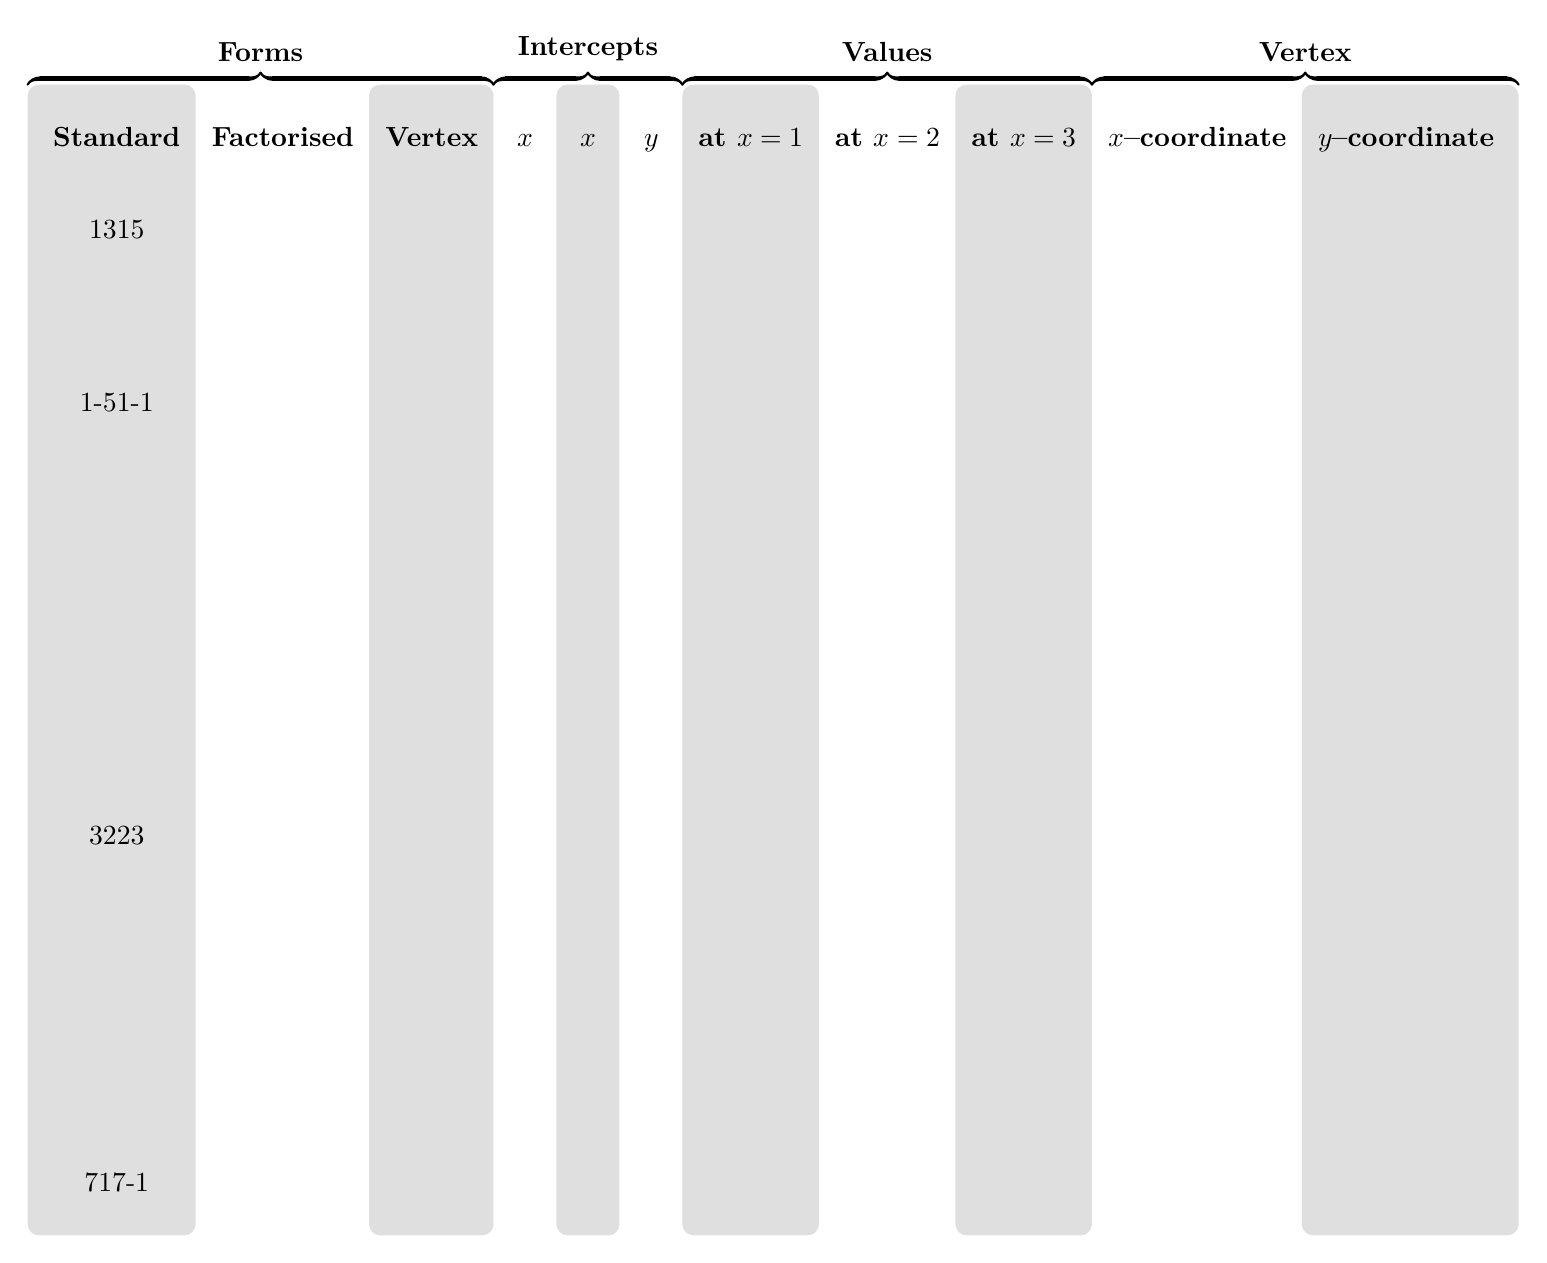
\begin{tikzpicture}
\matrix[
  matrix of nodes,
  ampersand replacement=\&,
  nodes={inner xsep=2mm, minimum width=.8cm,text opacity=0,minimum height=1.1cm},
  row 1/.style={every node/.append style={font=\bfseries,text opacity=1}},
  style odd tiling columns={fill=gray!25,rounded corners},
  %
  row 2/.style={every node/.append style={text opacity=1}},
  %
  row 3 column 2/.style={every node/.append style={text opacity=1}},
  row 4 column 1/.style={every node/.append style={text opacity=1}},
  row 5 column 3/.style={every node/.append style={text opacity=1}},
  row 6 column 4/.style={every node/.append style={text opacity=1}},
  row 6 column 5/.style={every node/.append style={text opacity=1}},
  row 6 column 6/.style={every node/.append style={text opacity=1}},
  row 7 column 7/.style={every node/.append style={text opacity=1}},
  row 7 column 8/.style={every node/.append style={text opacity=1}},
  row 7 column 9/.style={every node/.append style={text opacity=1}},
  row 8 column 2/.style={every node/.append style={text opacity=1}},
  row 9 column 1/.style={every node/.append style={text opacity=1}},
  row 10 column 3/.style={every node/.append style={text opacity=1}},
  row 11 column 4/.style={every node/.append style={text opacity=1}},
  row 11 column 5/.style={every node/.append style={text opacity=1}},
  row 11 column 6/.style={every node/.append style={text opacity=1}},
  row 12 column 2/.style={every node/.append style={text opacity=1}},
  row 13 column 1/.style={every node/.append style={text opacity=1}},
]
(m)
{
  Standard \&
  Factorised \&
  Vertex \&
  \(x\) \&
  \(x\) \&
  \(y\) \&
  at \(x = 1\) \&
  at \(x = 2\) \&
  at \(x = 3\) \&
  \(x\)--coordinate \&
  \(y\)--coordinate
  \\
  \QuadRow{1}{3}{1}{5}  \\ % 2
  \QuadRow{1}{2}{1}{3}  \\ % 3
  \QuadRow{1}{-5}{1}{-1}  \\ % 4
  \QuadRow{1}{3}{1}{-7}  \\ % 5
  \QuadRow{1}{-4}{1}{3} \\ % 6
  \QuadRow{1}{-1}{1}{3} \\ % 7
  \QuadRow{2}{3}{4}{5}  \\ % 8
  \QuadRow{3}{2}{2}{3}  \\ % 9
  \QuadRow{7}{-1}{5}{1}  \\ % 10
  \QuadRow{1}{-3}{1}{3}  \\ % 11
  \QuadRow{3}{-2}{3}{2}  \\ % 12
  \QuadRow{7}{1}{7}{-1}  \\ % 13
};
\draw[
  decorate,
  decoration={calligraphic brace,amplitude=1ex},
  ultra thick
] (m-tiling-cell-1-1.north west) -- node[above=1ex,font=\bfseries] {Forms} (m-tiling-cell-1-3.north east);
\draw[
  decorate,
  decoration={calligraphic brace,amplitude=1ex},
  ultra thick
] (m-tiling-cell-1-4.north west) -- node[above=1ex,font=\bfseries] {Intercepts} (m-tiling-cell-1-6.north east);
\draw[
  decorate,
  decoration={calligraphic brace,amplitude=1ex},
  ultra thick
] (m-tiling-cell-1-7.north west) -- node[above=1ex,font=\bfseries] {Values} (m-tiling-cell-1-9.north east);
\draw[
  decorate,
  decoration={calligraphic brace,amplitude=1ex},
  ultra thick
] (m-tiling-cell-1-10.north west) -- node[above=1ex,font=\bfseries] {Vertex} (m-tiling-cell-1-11.north east);
\end{tikzpicture}

\vspace*{\fill}


\end{document}
